\documentclass{beamer}
\bibliographystyle{amsalpha}
\usepackage{cite}
\usepackage[normalem]{ulem}
\usepackage{fancybox}
\usepackage{enumitem}
\setitemize{label=\usebeamerfont*{itemize item}
\usebeamercolor[fg]{itemize item}
  \usebeamertemplate{itemize item}}
\setbeamertemplate{footline}[frame number]{}
\setbeamertemplate{navigation symbols}{}
\graphicspath{{figures/}}

\title{Multi-Scale Plasma Modeling}
\subtitle{Combining Molecular Dynamics with Kinetic Theory}
\author[Price and Shohet]{Jake Price and Gil Shohet}
\institute[CPSSW]{Computational Physics Student Summer Workshop}
\date{August 5, 2015}


	\begin{document}
	
	\begin{frame}
	\maketitle
	\end{frame}
	
	\begin{frame}[t]{Personal Introduction}
	\begin{center}
\includegraphics[width=0.4\textwidth]{logo.png}\end{center}
	\vspace{-2em}
	\begin{columns}
	\column[t]{0.5\linewidth}
	\begin{center}\textbf{Research Interests}\end{center}
	\begin{itemize}
	\item Mesoscale simulation and modeling
	\item Stochastic analysis
	\item Mathematical biology
		\begin{itemize}
	\item Cellular biochemistry
	\item Nonequilibrium thermodynamics
	\end{itemize}
	\end{itemize}
	\column[t]{0.6\linewidth}
	\begin{center}
	\textbf{Future Directions}\vspace{0.575em}
	\begin{itemize}
	\item Heterogeneous multiscale method
	\begin{itemize}
	\item Plasma modeling
	\item Cellular biochemistry
	\end{itemize}
	\item Multiscale theory
	\begin{itemize}
	\item Numerical analysis
	\item Rigorous derivation of new methods
	\end{itemize}
	\end{itemize}
	\end{center}
	\end{columns}
		
	
	\end{frame}
	
	\begin{frame}{What is the Heterogeneous Multiscale Method (HMM)?}
		\begin{itemize}
		\item Most problems can be viewed on multiple scales\vspace{1em}
		\item HMM is a \textbf{top-down} strategy for creating a \textbf{hybrid method} that uses the microscale model to increase the accuracy of the macroscale model
		\end{itemize}
		
		\begin{center}
			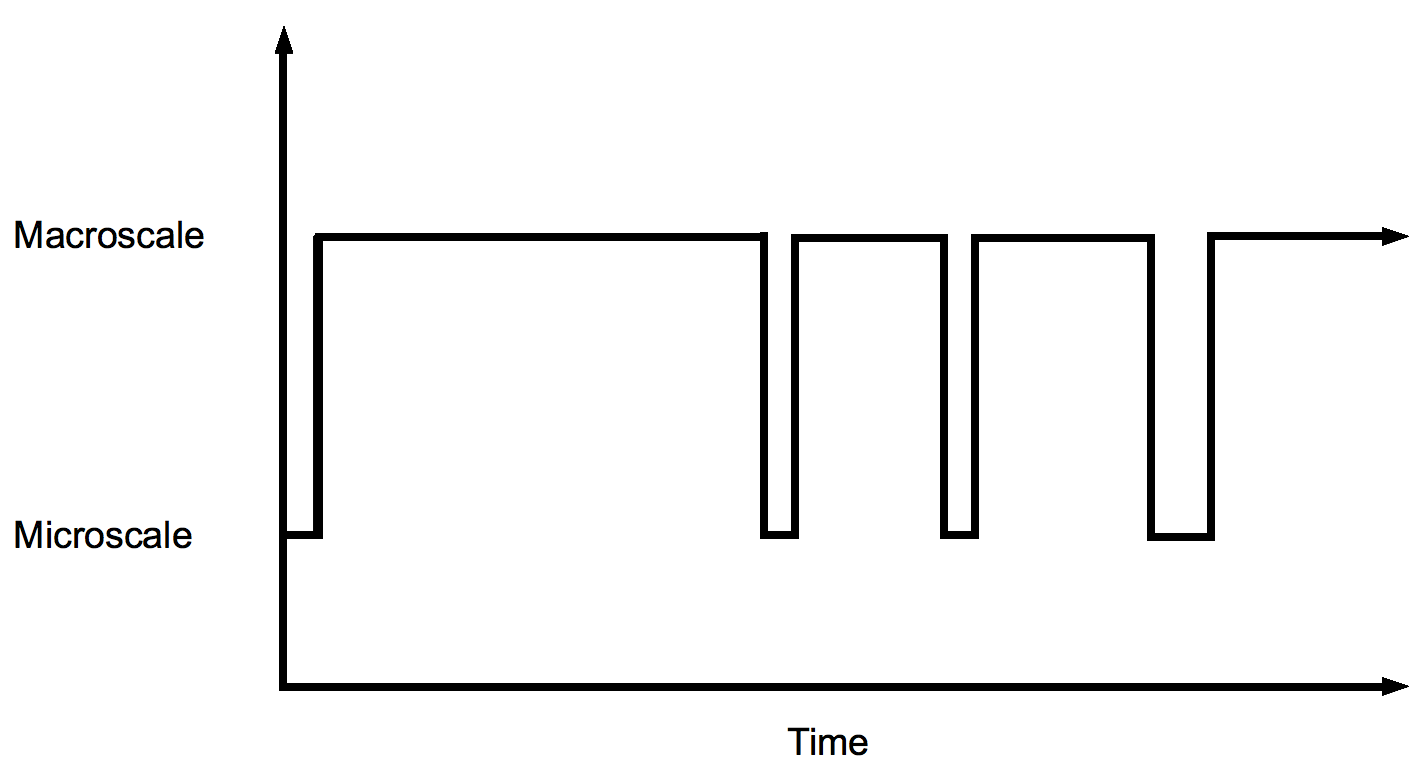
\includegraphics[height = 0.5\textheight]{scheme.png}
			\end{center}
	\end{frame}
	
	\begin{frame}{Our Goal}
		\begin{itemize}
			\item  Develop a proof-of-concept computational framework to model plasmas using HMM\vspace{1em}
			\begin{itemize}
			\item  Macroscopic model: Kinetic theory using the BGK approximation of the Boltzmann equation\vspace{1em}
		
			\item  Microscopic model: Molecular dynamics\vspace{1em}
			\end{itemize}
			\item  The mathematical framework is built up from first principles and is designed to be as general as possible
		\end{itemize}
	\end{frame}
	
	\begin{frame}[t]{Connecting the Models}
\hspace{1.75em}\textbf{Molecular Dynamics}\hspace{4.5em}\textbf{BGK Kinetic Theory}
			
		\vspace{0.5em}
		\begin{center}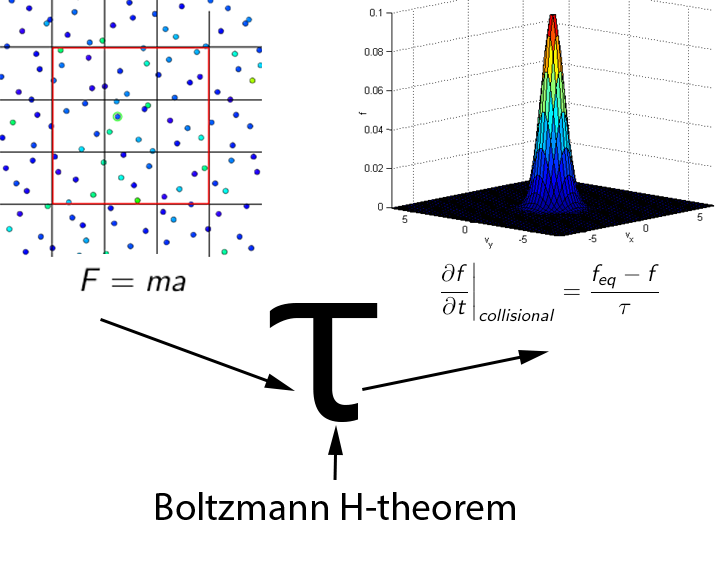
\includegraphics[width=0.85\textwidth]{model_link.png}\end{center}
	\end{frame}
		
\end{document}